\documentclass[pdf]{beamer}

%\usepackage{lmodern}
\usepackage[font=scriptsize,skip=0pt,justification=justified,singlelinecheck=false]{caption}
%\usepackage{enumitem}
\usepackage{natbib}
\usepackage{bm}
\usepackage{mathtools}
\usepackage[makeroom]{cancel}
\usepackage{minted}

% Using underline
\usepackage{soul}

\usepackage{algorithm}
\usepackage{algpseudocode}
%\usepackage[ruled,vlined]{algorithm2e}
%\usepackage{clrscode3e}


%\usepackage{adjustbox}

%remove the icon
\setbeamertemplate{bibliography item}{}

%remove line breaks
\setbeamertemplate{bibliography entry title}{}
\setbeamertemplate{bibliography entry location}{}
\setbeamertemplate{bibliography entry note}{}
% Use number for caption
\setbeamertemplate{caption}[numbered]{}

\newtheorem{mydef}[theorem]{\Large \underline{\textbf{Definisi}}}

\makeatletter
\def\th@mystyle{%
    \normalfont % body font
    \setbeamercolor{block title example}{bg=blue,fg=white}
    \setbeamercolor{block body example}{bg=blue!20,fg=black}
    \def\inserttheoremblockenv{exampleblock}
  }
\makeatother
\theoremstyle{mystyle}
\newtheorem*{remark}{\textbf{Definition}}


% This file is a solution template for:

% - Talk at a conference/colloquium.
% - Talk length is about 20min.
% - Style is ornate.

% Copyright 2004 by Till Tantau <tantau@users.sourceforge.net>.
%
% In principle, this file can be redistributed and/or modified under
% the terms of the GNU Public License, version 2.
%
% However, this file is supposed to be a template to be modified
% for your own needs. For this reason, if you use this file as a
% template and not specifically distribute it as part of a another
% package/program, I grant the extra permission to freely copy and
% modify this file as you see fit and even to delete this copyright
% notice.  


\mode<presentation>
{
%  \usetheme{AnnArbor} % 
%	\usetheme{Frankfurt}
   \usetheme{Madrid}
  % or ...

%  \setbeamercovered{transparent}
  % or whatever (possibly just delete it)
}


\usepackage[english]{babel}
% or whatever

\usepackage[latin1]{inputenc}
% or whatever

\usepackage{times}
\usepackage[T1]{fontenc}
\usepackage{wasysym}

\usepackage{graphicx} % Necessary to use \scalebox

% Define absolute and norm
\DeclarePairedDelimiter\abs{\lvert}{\rvert}%
\DeclarePairedDelimiter\norm{\lVert}{\rVert}%

% ==============================
%       Redefine emphasize
% ==============================
\let\emph\relax % there's no \RedeclareTextFontCommand
\DeclareTextFontCommand{\emph}{\bfseries\em}


% Swap the definition of \abs* and \norm*, so that \abs
% and \norm resizes the size of the brackets, and the 
% starred version does not.
\makeatletter
\let\oldabs\abs
\def\abs{\@ifstar{\oldabs}{\oldabs*}}
%
\let\oldnorm\norm
\def\norm{\@ifstar{\oldnorm}{\oldnorm*}}
\makeatother

\usepackage{color}
\definecolor{myblue}{rgb}{.8,.8,1}
\usepackage{empheq}
% Or whatever. Note that the encoding and the font should match. If T1
% does not look nice, try deleting the line with the fontenc.

\newlength\mytemplen
\newsavebox\mytempbox

\makeatletter
\newcommand\mybluebox{%
    \@ifnextchar[%]
       {\@mybluebox}%
       {\@mybluebox[0pt]}}

\def\@mybluebox[#1]{%
    \@ifnextchar[%]
       {\@@mybluebox[#1]}%
       {\@@mybluebox[#1][0pt]}}

\def\@@mybluebox[#1][#2]#3{
    \sbox\mytempbox{#3}%
    \mytemplen\ht\mytempbox
    \advance\mytemplen #1\relax
    \ht\mytempbox\mytemplen
    \mytemplen\dp\mytempbox
    \advance\mytemplen #2\relax
    \dp\mytempbox\mytemplen
    \colorbox{myblue}{\hspace{1em}\usebox{\mytempbox}\hspace{1em}}}

\makeatother

\title[AI untuk Semua] % (optional, use only with long paper titles)
{\textbf{Pengenalan Topik Kecerdasan Buatan}}

\subtitle
{AI for everyone\footnote{https://www.coursera.org/learn/ai-for-everyone/home/welcome}}

\author[Hendra Bunyamin] % (optional, use only with lots of authors)
{Hendra Bunyamin}
%{F.~Author\inst{1} \and S.~Another\inst{2}} --> original
% - Give the names in the same order as the appear in the paper.
% - Use the \inst{?} command only if the authors have different
%   affiliation.

\institute[ ] % (optional, but mostly needed)
{
%  \inst{1}%
  Jurusan Teknik Informatika\\
  Fakultas Teknologi Informasi\\
  Universitas Kristen Maranatha
%  \and
%  \inst{2}%
%  Department of Theoretical Philosophy\\
%  University of Elsewhere
}
% - Use the \inst command only if there are several affiliations.
% - Keep it simple, no one is interested in your street address.

%\date[CFP 2003] % (optional, should be abbreviation of conference name)
%{Conference on Fabulous Presentations, 2003}
% - Either use conference name or its abbreviation.
% - Not really informative to the audience, more for people (including
%   yourself) who are reading the slides online

\subject{Pengantar Teknologi Informasi}
% This is only inserted into the PDF information catalog. Can be left
% out. 

% If you have a file called "university-logo-filename.xxx", where xxx
% is a graphic format that can be processed by latex or pdflatex,
% resp., then you can add a logo as follows:

\pgfdeclareimage[height=1.5cm]{university-logo}{logo-mcu}
\logo{\pgfuseimage{university-logo}}


% Delete this, if you do not want the table of contents to pop up at
% the beginning of each subsection:
\AtBeginSection[]
{
  \begin{frame}<beamer>{Outline}
    \tableofcontents[currentsection,currentsection]
  \end{frame}
}


% If you wish to uncover everything in a step-wise fashion, uncomment
% the following command: 

%\beamerdefaultoverlayspecification{<+->}

\begin{document}

\begin{frame}
  \titlepage
\end{frame}

\begin{frame}{Outline}
  \tableofcontents
  % You might wish to add the option [pausesections]
\end{frame}


% Structuring a talk is a difficult task and the following structure
% may not be suitable. Here are some rules that apply for this
% solution: 

% - Exactly two or three sections (other than the summary).
% - At *most* three subsections per section.
% - Talk about 30s to 2min per frame. So there should be between about
%   15 and 30 frames, all told.

% - A conference audience is likely to know very little of what you
%   are going to talk about. So *simplify*!
% - In a 20min talk, getting the main ideas across is hard
%   enough. Leave out details, even if it means being less precise than
%   you think necessary.
% - If you omit details that are vital to the proof/implementation,
%   just say so once. Everybody will be happy with that.

%\begin{frame}{Make Titles Informative. Use Uppercase Letters.}{Subtitles are optional.}

\section{Introduction}
\begin{frame}{Introduction}
	\begin{figure}[!ht]
		\centering
		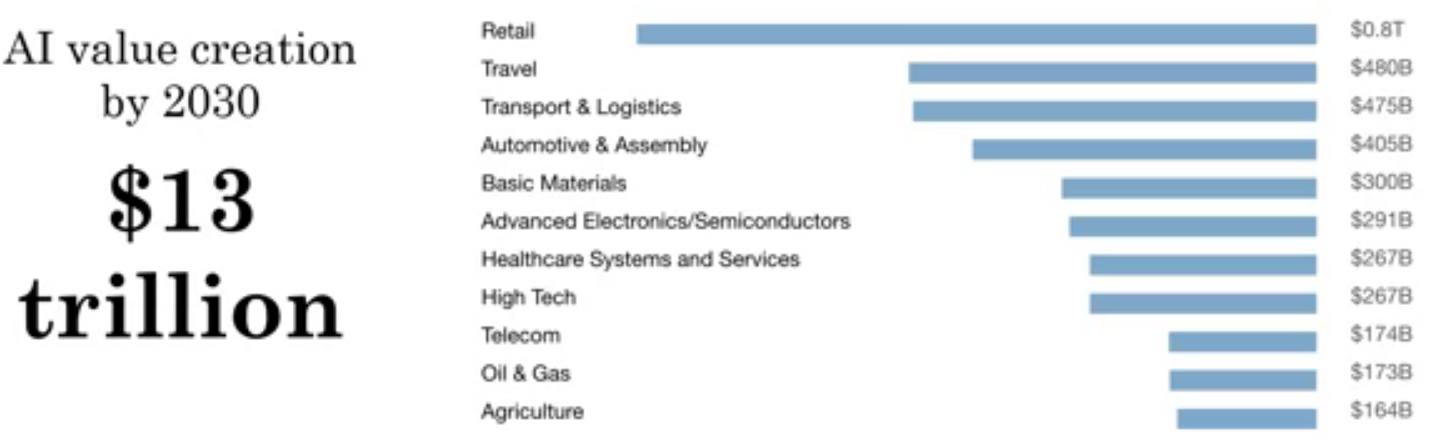
\includegraphics[scale=.225]{AI-value-creation}
		\caption{Source: McKinsey Global Institute~\citep{ng2019AIForEveryone}}
		\label{fig:ai-value-creation}
	\end{figure}
	\$$13$ trillion = \$$13 \times 10^{12} = \text{Rp}183 \times 10^{15}$. 
\end{frame}

\begin{frame}{Demystifying AI}
	Artificial Intelligence or \textbf{AI} can be divided into 2 as follows:
	\begin{itemize}
		\item \textbf{ANI} $\Rightarrow$ Artificial Narrow Intelligence. \\
		Examples: smart speaker, self-driving car, web search, AI in farming and factories.
		\bigskip
		\item \textbf{AGI} $\Rightarrow$ Artificial General Intelligence. \\
		Examples: Do anything a human can do atau bahkan melebihi.
	\end{itemize}
	\begin{center}
		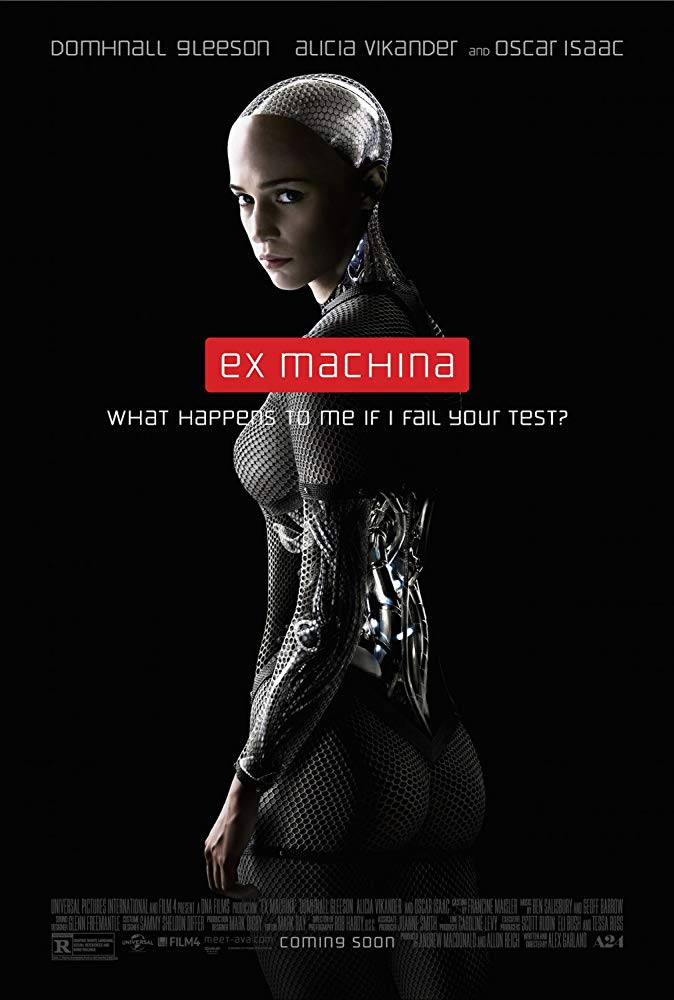
\includegraphics[scale=.125]{ex-machina} \qquad 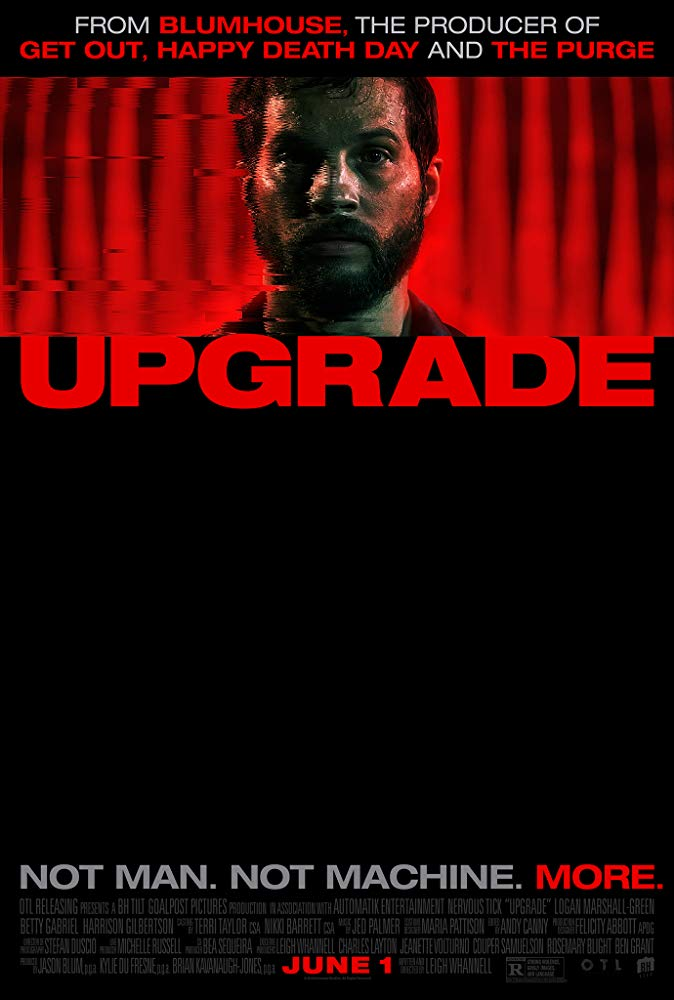
\includegraphics[scale=.125]{upgrade}
	\end{center}
	
\end{frame}

\section{Machine Learning}
\begin{frame}{Supervised Learning (1/2)}
	\begin{itemize}
		\item One of the tools that drive the significant progress of AI is \textbf{Machine Learning}.
		
		\bigskip		
		
		\item A common type of of Machine Learning is a type of AI that learns from $A$ to $B$	or is often called \emph{Supervised Learning}.
		
		\bigskip
		
		\begin{center}
			
			\scalebox{2}{
				$A \longrightarrow B$
			} \\	
			\scalebox{1}{
				\qquad input \qquad \; \; output
			}							
		\end{center}
	\end{itemize}	
\end{frame}


\begin{frame}{Supervised Learning (2/2)}
	\begin{table}[!ht]
		\centering
		\begin{tabular}{ccc|l}
			\textbf{Input ($\bm{A}$)} &  & \textbf{Output ($\bm{B}$)} & \textbf{Application} \\
			\hline
			email     & $\longrightarrow$  & spam? (0/1)                & spam filtering   \\
			          &                    &                            &                  \\
			audio     & $\longrightarrow$  & text transcript            & speech recognition      \\
			          &                    &                            &                  \\
			English   & $\longrightarrow$  & Indonesia                  & machine translation \\
			          &                    &                            &                  \\
			ad, user info & $\longrightarrow$ & click? (0/1)            & online advertising \\
			          &                    &                               &                  \\
			image, radar info & $\longrightarrow$ & position of other cars &  self-driving car \\
			          &                    &                               &                  \\
			image of phone & $\longrightarrow$ & defect? (0/1)             & visual inspection \\
			\hline           			             
		\end{tabular}
	\end{table}
\end{frame}

\begin{frame}{Why Now?}
	\begin{figure}[!ht]
		\centering
		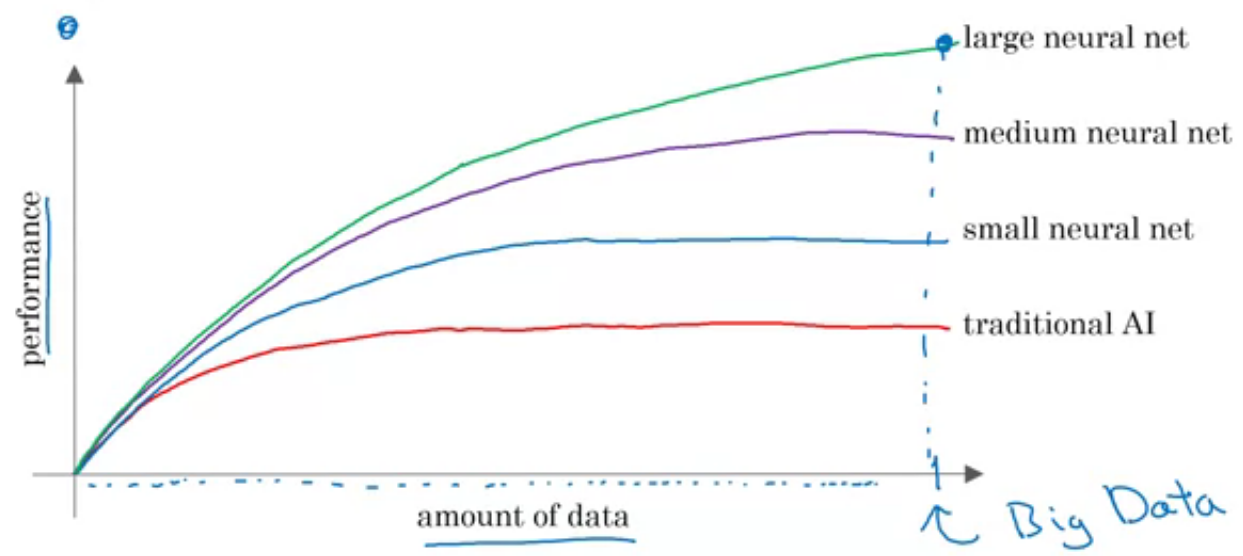
\includegraphics[scale=.25]{big-data}
		\caption{Large neural net + Big Data = High Performance~\citep{ng2019AIForEveryone}}
		\label{fig:big-data}
	\end{figure}
\end{frame}

\section{What is Data?}
\begin{frame}{Example of a Table of Data (Dataset) (1/3)}
	\begin{table}[!ht]
		\centering
		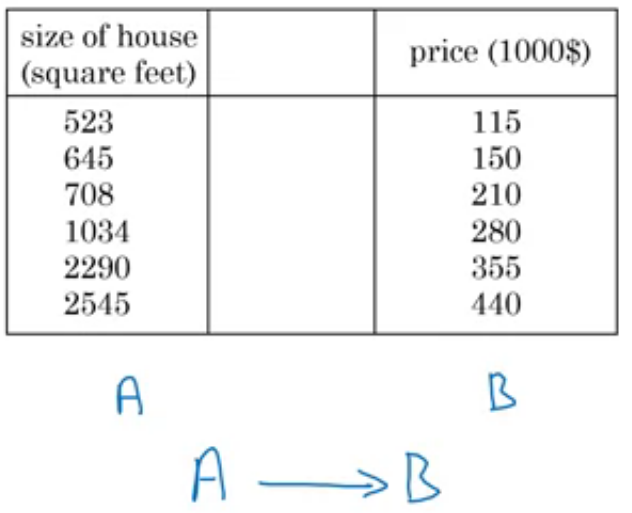
\includegraphics[scale=.3]{example-dataset-2}
		\caption{House prices dataset~\citep{ng2019AIForEveryone}}
		\label{fig:example-dataset-2}
	\end{table}
\end{frame}


\begin{frame}{Example of a Table of Data (Dataset) (2/3)}
	\begin{table}[!ht]
		\centering
		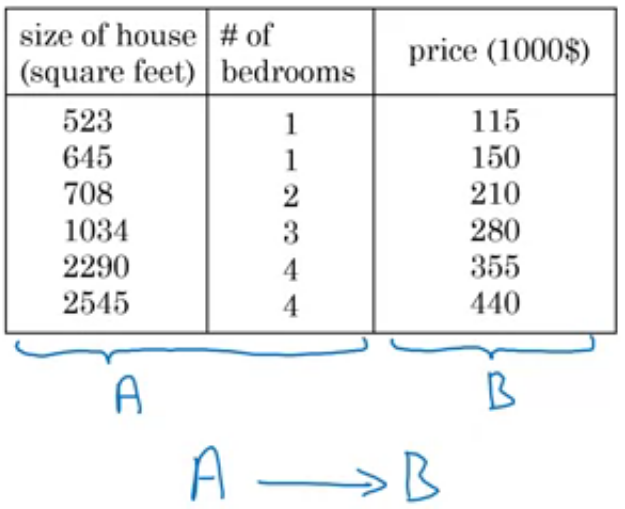
\includegraphics[scale=.3]{example-dataset-1}
		\caption{House prices dataset~\citep{ng2019AIForEveryone}}
		\label{fig:example-dataset-1}
	\end{table}
\end{frame}

\begin{frame}{Example of a Table of Data (Dataset) (3/3)}
	\begin{table}[!ht]
		\centering
		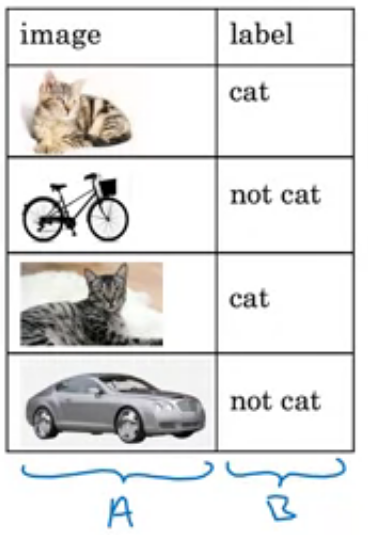
\includegraphics[scale=.3]{example-dataset-3}
		\caption{Cat images dataset~\citep{ng2019AIForEveryone}}
		\label{fig:example-dataset-3}
	\end{table}
\end{frame}

\begin{frame}{Acquiring data}
	\begin{itemize}
		\item Manual labeling
		\begin{center}
			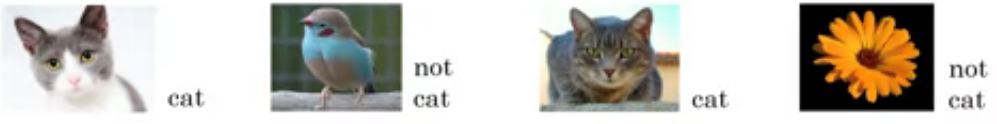
\includegraphics[scale=.3]{manual-labeling}
		\end{center}
		\item From observing behaviors
		\begin{center}
			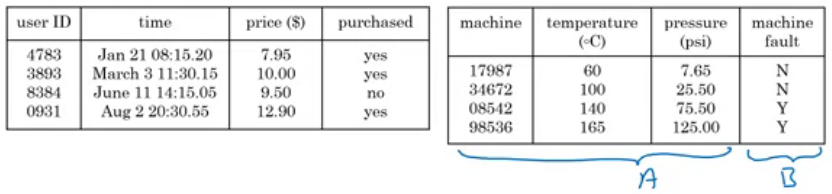
\includegraphics[scale=.35]{observing-behaviors}
		\end{center}
		\item Download from websites / partnerships		
	\end{itemize}
\end{frame}

\begin{frame}{Data is Messy}
	\begin{itemize}
		\item Garbage in, garbage out
		\item Data problems: \textit{incorrect labels} and \textit{missing values} 
		\begin{center}
			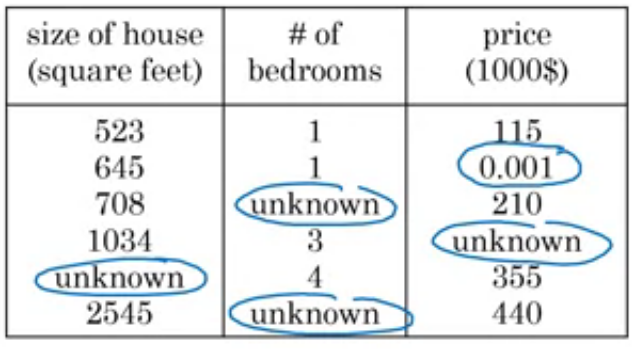
\includegraphics[scale=.3]{data-problems} 
		\end{center}
		\item Multiple types of data \\
		\textit{images}, \textit{audio}, \textit{text} $\Rightarrow$ \textbf{unstructured data}					
	\end{itemize}
\end{frame}

\section{The Terminology of AI}
\begin{frame}{Machine Learning vs. Data Science (1/2)}
	\begin{figure}[!ht]
		\centering
		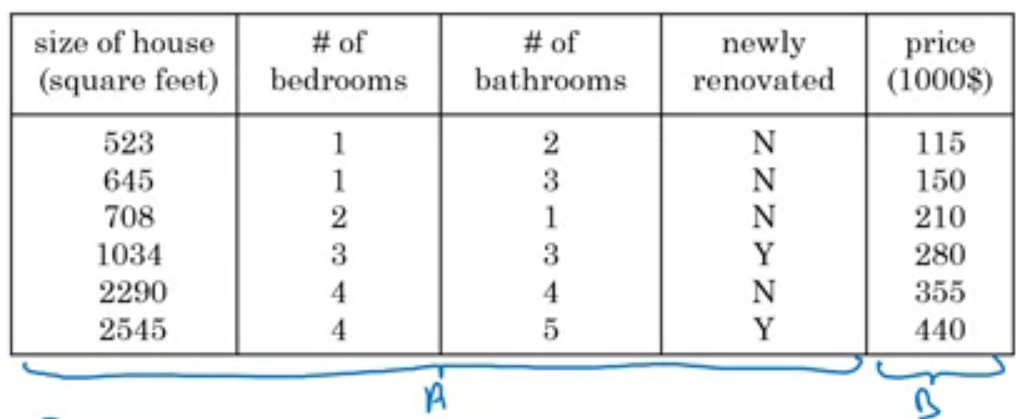
\includegraphics[scale=.25]{ml-vs-ds}		
		\caption{Home prices~\citep{ng2019AIForEveryone}}
	\end{figure}
	\vspace*{-.5cm}
	\textbf{According to \textit{Machine Learning}}: \\
	$A \longrightarrow B$: Running AI system (e.g., websites / mobile app) \\		
	\textbf{According to \textit{Data Science}}: \\
	\textit{Homes with 3 bedrooms are more expensive than homes with 2 bedrooms of a similar size}. \\		
	\textit{Newly renovated homes have a 15\% premium}.
\end{frame}

\begin{frame}{Machine Learning vs. Data Science (2/2)}
	\begin{table}[!ht]
		\centering
		\begin{tabular}{cc}
			\textbf{Machine Learning}        & \textbf{Data Science} \\
			                                 &                       \\
			 "Field of study that gives     & Science of extracting knowledge \\
			 computers the ability to learn  & and insights from data. \\
			 without being explicitly        &   \\
			 programmed."                    &   \\
			 $\longrightarrow$ software      & $\longrightarrow$ slide deck  \\
			 -Arthur Samuel (1959)           & 
		\end{tabular}
	\end{table}
\end{frame}



\begin{frame}{Deep Learning (1/2)}
	\begin{center}
		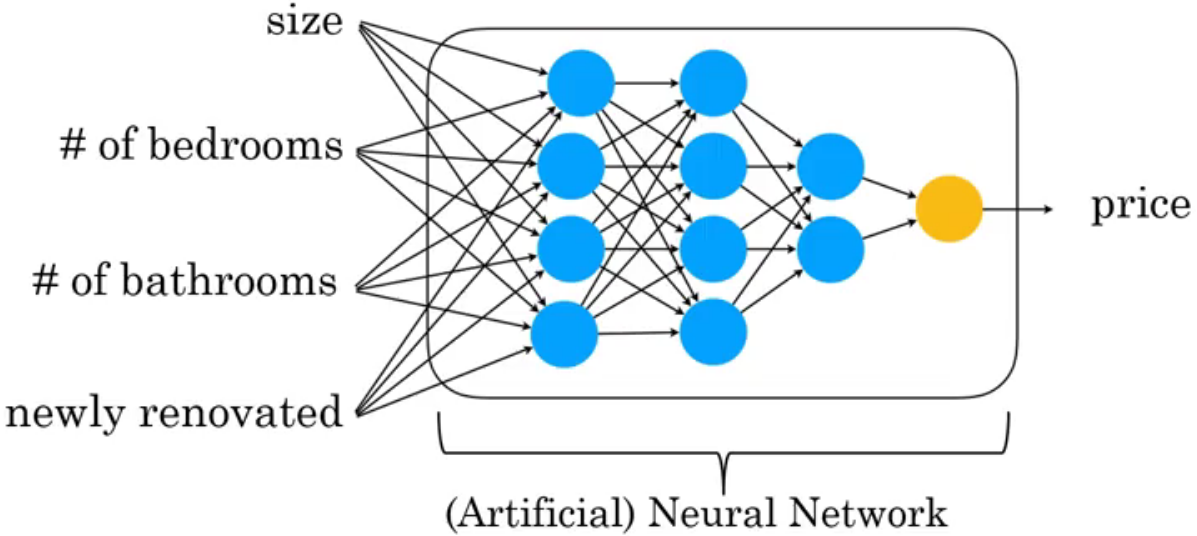
\includegraphics[scale=.275]{deep-learning}
	\end{center}	
\end{frame}

\begin{frame}{Deep Learning (2/2)}
	\begin{center}
		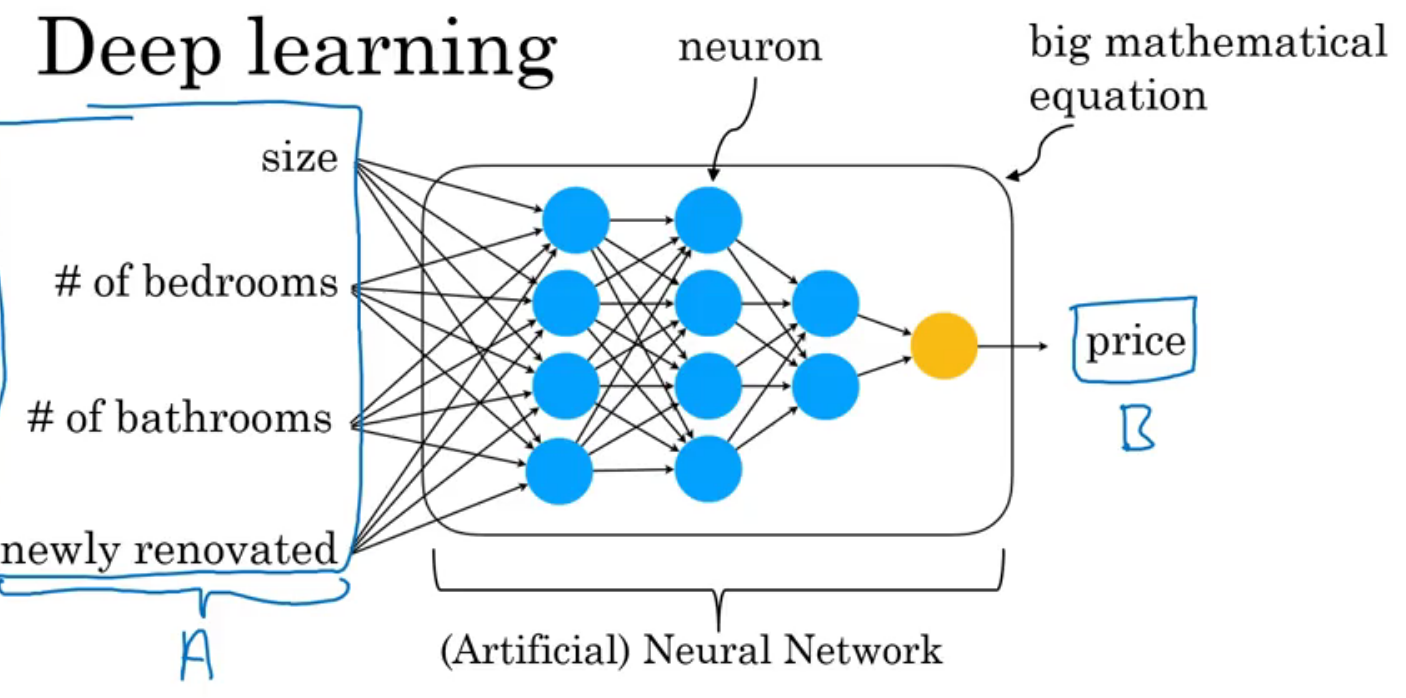
\includegraphics[scale=.24]{deep-learning-2}
	\end{center}	
\end{frame}

\begin{frame}{AI has many tools (1/2)}
	\begin{itemize}
		\item Machine learning and data science
		
		\bigskip		
		
		\item Deep learning / neural network 
		
		\bigskip
		
		\item Other buzzwords: Unsupervised learning, reinforcement learning, graphical models, planning, knowledge graph, ...
	\end{itemize}
\end{frame}

\begin{frame}{AI has many tools (2/2)}
	\begin{figure}[!ht]
		\centering
		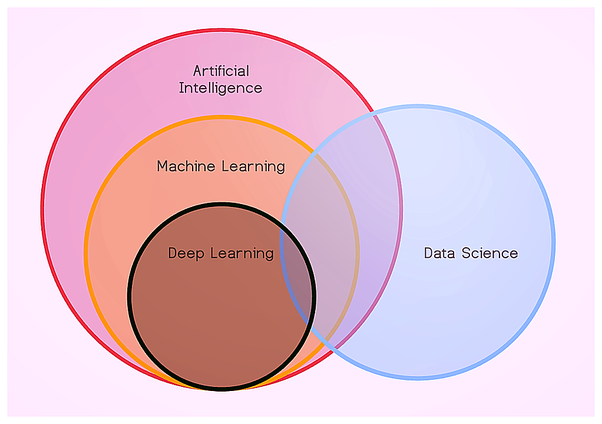
\includegraphics[scale=.45]{diagram-venn-deep-learning}
		\caption{Relationship among AI, ML, DL, and DS~\citep{kharkovyna2019ABeginnersGuide}}
	\end{figure}
\end{frame}

\section{What Machine Learning Can and Cannot Do}
\begin{frame}{Supervised Learning}
	\begin{center}
		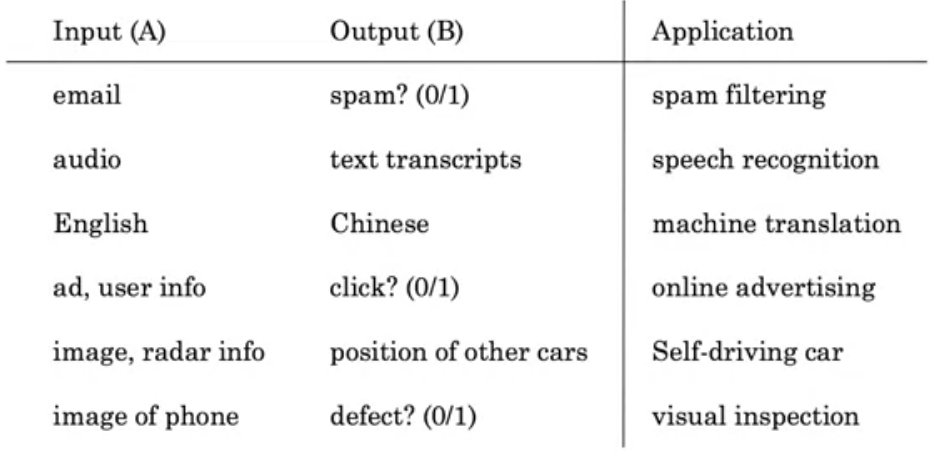
\includegraphics[scale=.3]{what-ML-can-do}
	\end{center}
	\begin{center}
		Anything you can do with 1 second of thought, we can probably now or soon automate.
	\end{center}
\end{frame}

\begin{frame}{What machine learning today can and cannot do}
	The toy arrived two days late, so I wasn't able to give it to my niece for her birthday. \\
	Can I return it?

	\bigskip
	
	$\longrightarrow$ "\textit{Refund request}" \\
	Input text $\longrightarrow$ Refund/Shipping/Other \\
	$A \longrightarrow B$
	
	\bigskip
	
	$\longrightarrow$ "\textit{Oh, sorry to hear that. I hope your niece had a good birthday. Yes, we can help with ...}"	
	
\end{frame}

\begin{frame}{What happens if you try?}
	\begin{tabular}{lcl}
		\textbf{Input (A)} & $\longrightarrow$ & \textbf{Output (B)} \\
		User email	       &                   & 2-3 paragraph response
	\end{tabular}

	\bigskip
	
	1000 examples 
	
	\bigskip
	
	\begin{tabular}{lcl}
		"My box was damaged" & $\longrightarrow$ & Thank you for your email. \\
		   	                 &                     &   \\
		"Where do I write a review?" & $\longrightarrow$ & Thank you for your email. \\		   	                 
		   	                 &                     &   \\
		"What's the return policy" & $\longrightarrow$ & Thank you for your email. \\		   	                 		   	                 		   	                 &                     &   \\
		"When is my box arriving?" & $\longrightarrow$ & Thank yes now your....
	\end{tabular}
\end{frame}
	
\begin{frame}{What makes an ML problem easier}
	\begin{enumerate}
		\item Learning a "simple" concept \\
		\begin{center}
			
			\scalebox{2}{
				$\leq 1 \text{ sec}$
			} 							
		\end{center}		
		
		\bigskip		
		
		\item Lots of data available \\
		\begin{center}
			
			\scalebox{2}{
				$A \longrightarrow B$
			} \\	
			\scalebox{1}{
				\qquad input \qquad \; \; output
			}							
		\end{center}				
	\end{enumerate}
\end{frame}	

\section{More examples of what ML can and cannot do}
\begin{frame}{Self-driving car}
	\begin{columns}[c]		
		\begin{column}{0.5\textwidth}
			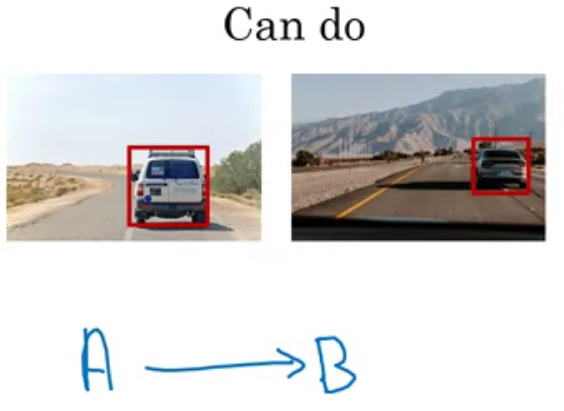
\includegraphics[scale=.225]{kiri-can}
			\vspace*{1.75cm}
		\end{column}
		\hspace{-50pt}
		\vrule{}
		\begin{column}{0.5\textwidth}
			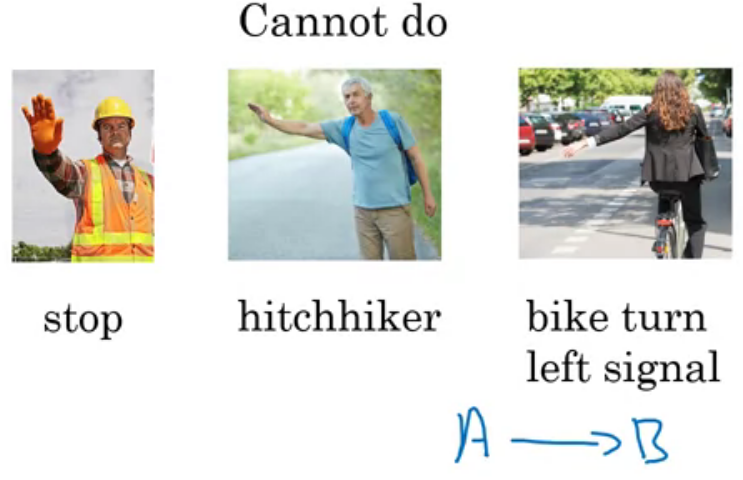
\includegraphics[scale=.225]{kanan-can}				
	\begin{enumerate}
		\item Data 
		\item Need high accuracy
	\end{enumerate}					
		\end{column}		
	\end{columns}	
\end{frame}
	
\begin{frame}{X-ray diagnosis}
	\begin{center}
		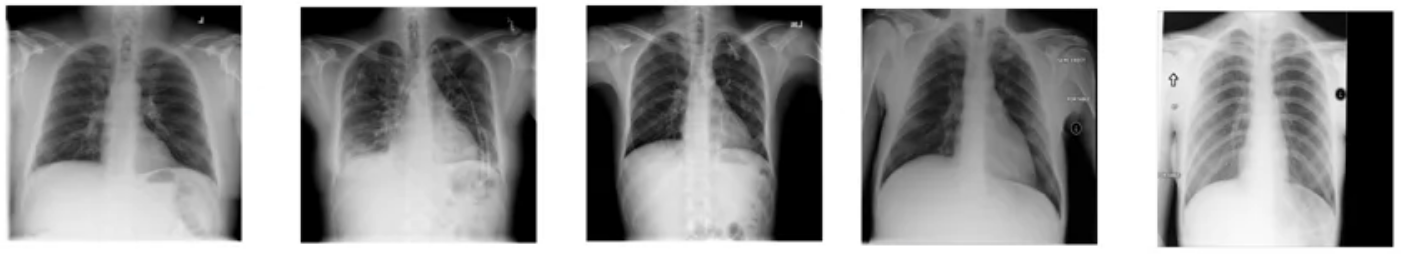
\includegraphics[scale=.225]{x-ray}	
	\end{center}		
	\centering
	\begin{tabular}{l|l}
		\multicolumn{1}{c|}{\textbf{Can do}} & \multicolumn{1}{c}{\textbf{Cannot do}} \\
		                                    &   \\
	    Diagnose pneumonia from                      &    Diagnose pneumonia from \\
	    $\thicksim$10,000 labeled images             &    10 images of medical textbook \\
	                                                 &    chapter explaining pneumonia	                  
	\end{tabular}	
\end{frame}

\begin{frame}{Strengths and weaknesses of machine learning}
	ML tends to work well when:
	\begin{enumerate}
		\item Learning a "simple" concept 
		\item There are lots of data available
	\end{enumerate}
	
	\bigskip	
	
	ML tends to work poorly when:
	\begin{enumerate}
		\item Learning complex concepts from small amounts of data
		\item It is asked to perform on new types of data
	\end{enumerate}
	\begin{center}
		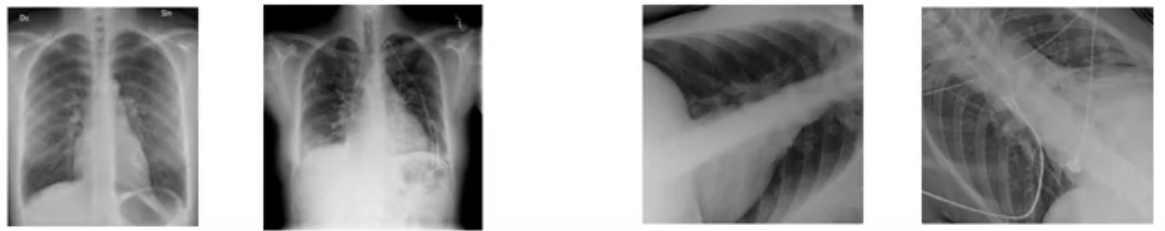
\includegraphics[scale=.275]{new-types-of-data}
	\end{center}
\end{frame}
	
\section{Non-technical explanation of deep learning}
\begin{frame}{Demand prediction (1/2)}
	\begin{columns}[c]		
		\begin{column}{0.6\textwidth}
			\hspace{20pt}
			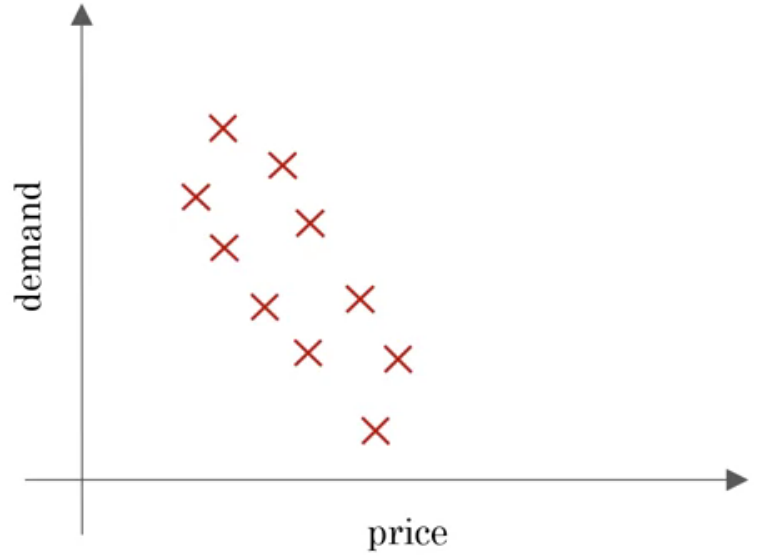
\includegraphics[scale=.225]{demand-prediction}
		\end{column}
		\hspace{-10pt}
		\begin{column}{0.4\textwidth}
			
\includegraphics[scale=.225]{t-shirt}				
		\end{column}		
	\end{columns}	
\end{frame}

\begin{frame}{Demand prediction (2/2)}
	\centering
	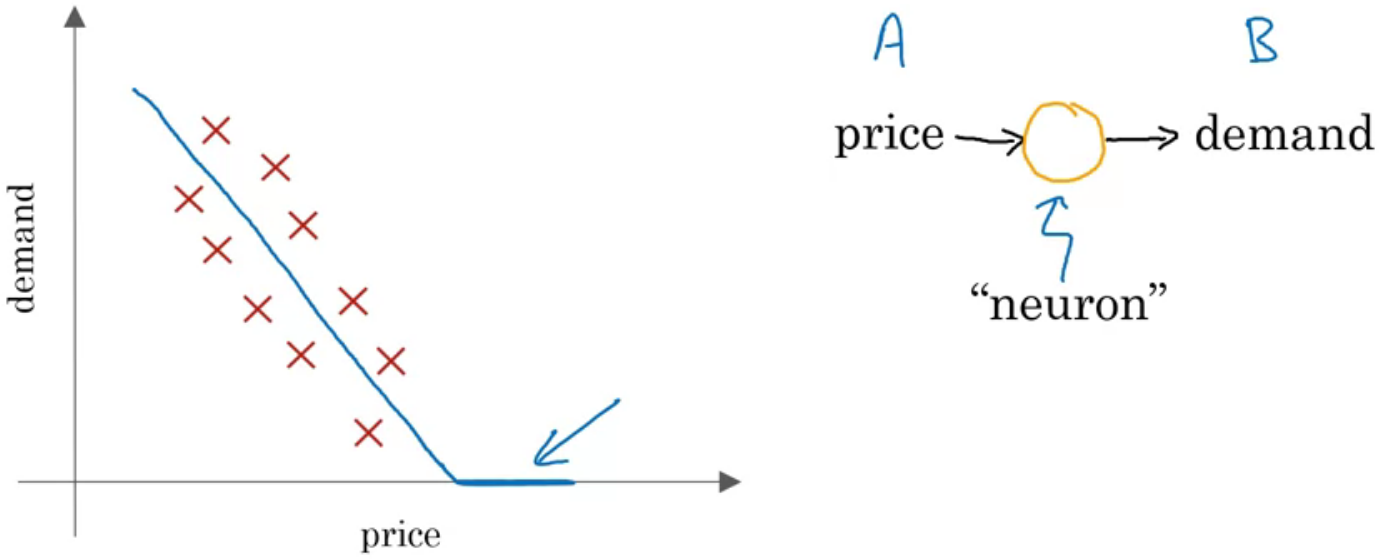
\includegraphics[scale=.225]{demand-prediction-line}
\end{frame}

\begin{frame}{Demand prediction: a little bit more complex (1/3)}
	\centering
	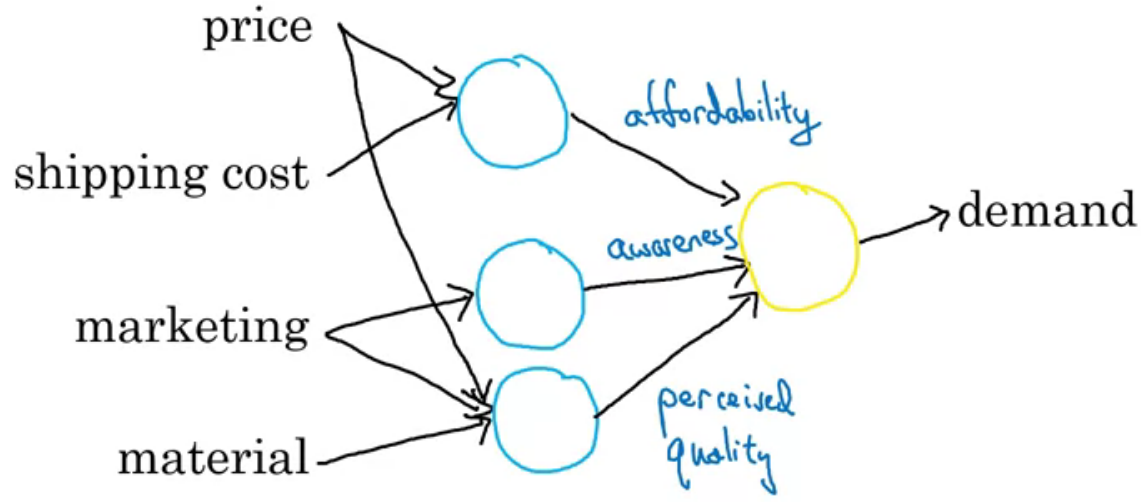
\includegraphics[scale=.275]{demand-prediction-nn.png}
\end{frame}

\begin{frame}{Demand prediction: a little bit more complex (2/3)}
	\centering
	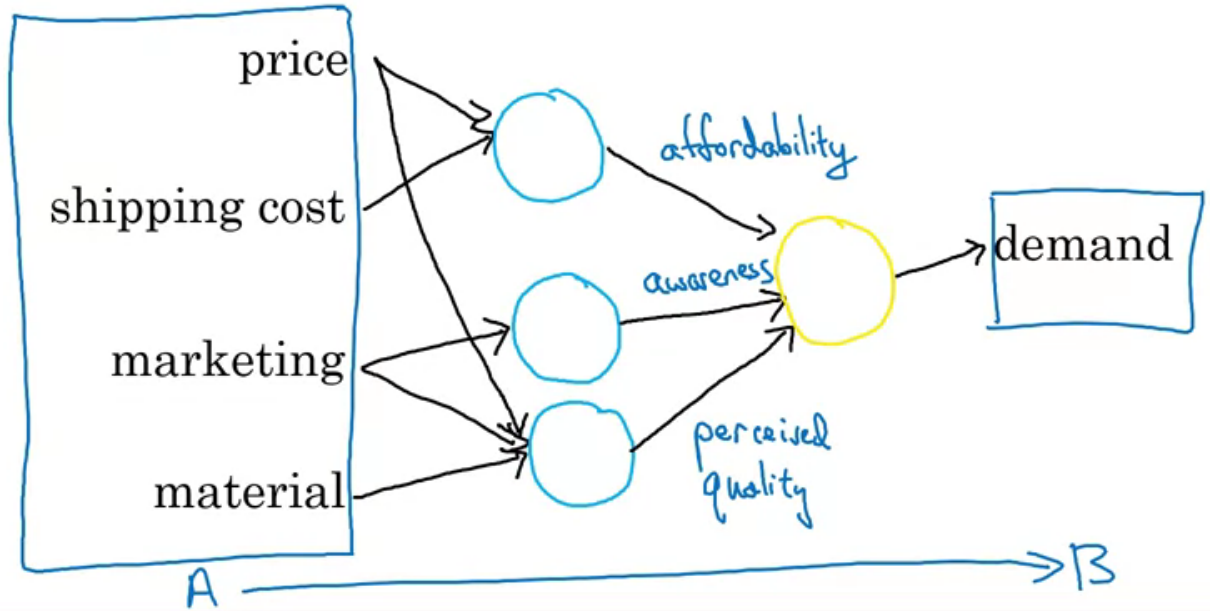
\includegraphics[scale=.275]{demand-prediction-nn-2.png}
\end{frame}

\begin{frame}{Demand prediction: a little bit more complex (3/3)}
	\centering
	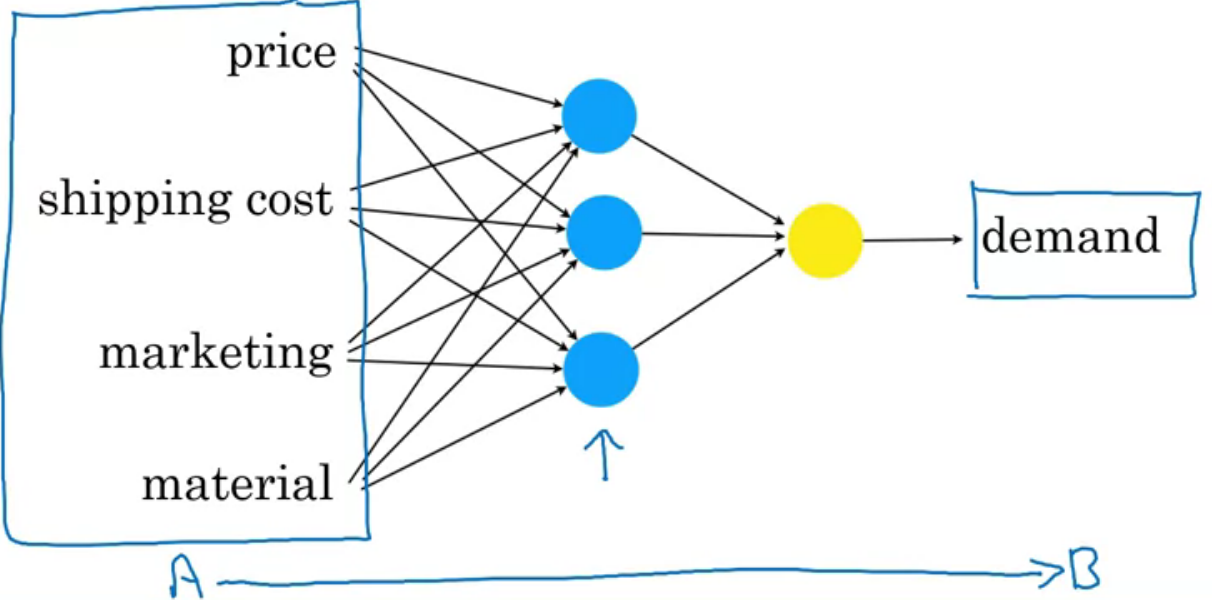
\includegraphics[scale=.275]{demand-prediction-nn-3.png}
\end{frame}

\begin{frame}{NN Application: Face recognition (1/3)}
	We want to build a system that recognizes people from pictures.
	\begin{figure}[!ht]
		\centering
		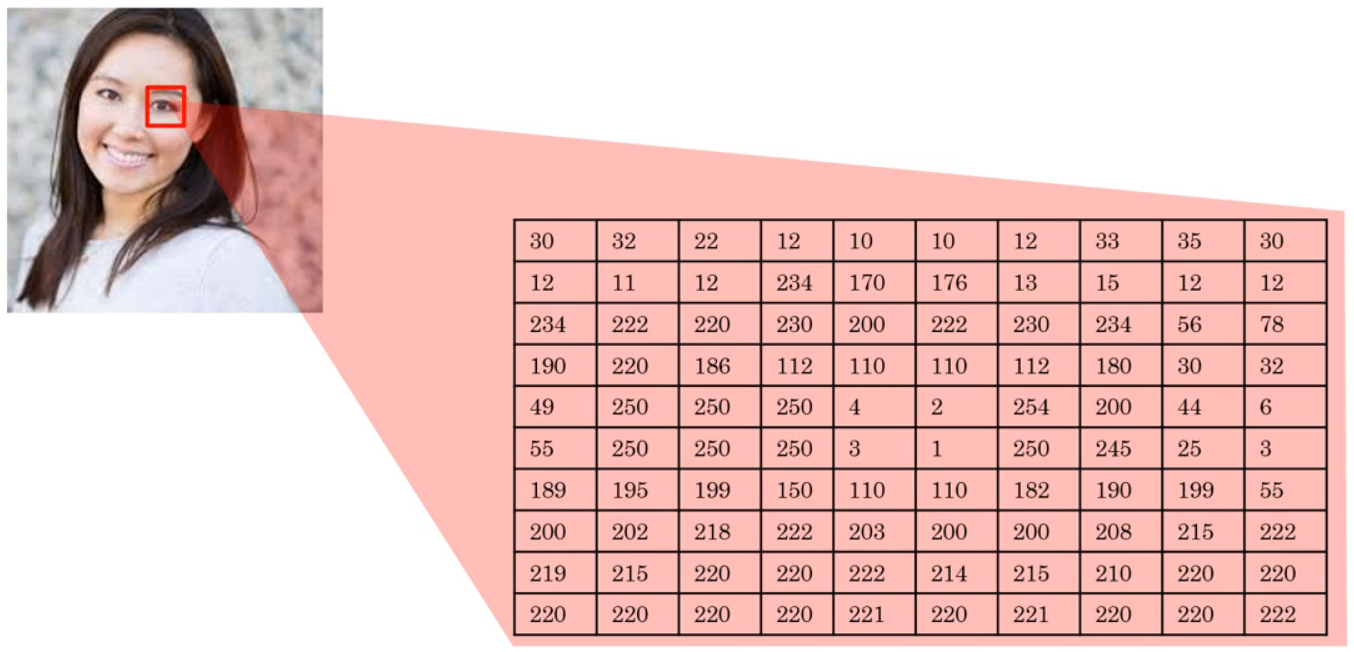
\includegraphics[scale=.25]{face-recognition-intro}
		\caption{What a computer sees from an image (assume the picture is grayscale)~\citep{ng2019AIForEveryone}}
	\end{figure}
	
\end{frame}

\begin{frame}{NN Application: Face recognition (2/3)}
		\centering
		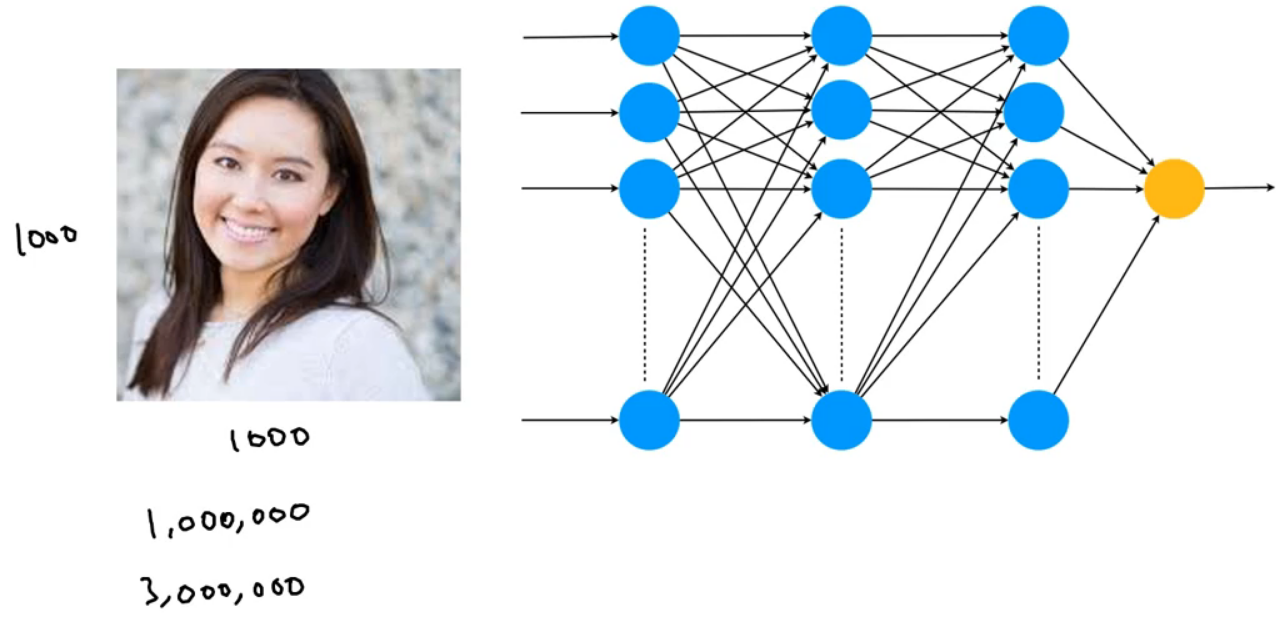
\includegraphics[scale=.25]{face-recognition-intro-2}
\end{frame}

\begin{frame}{NN Application: Face recognition (3/3)}
		\centering
		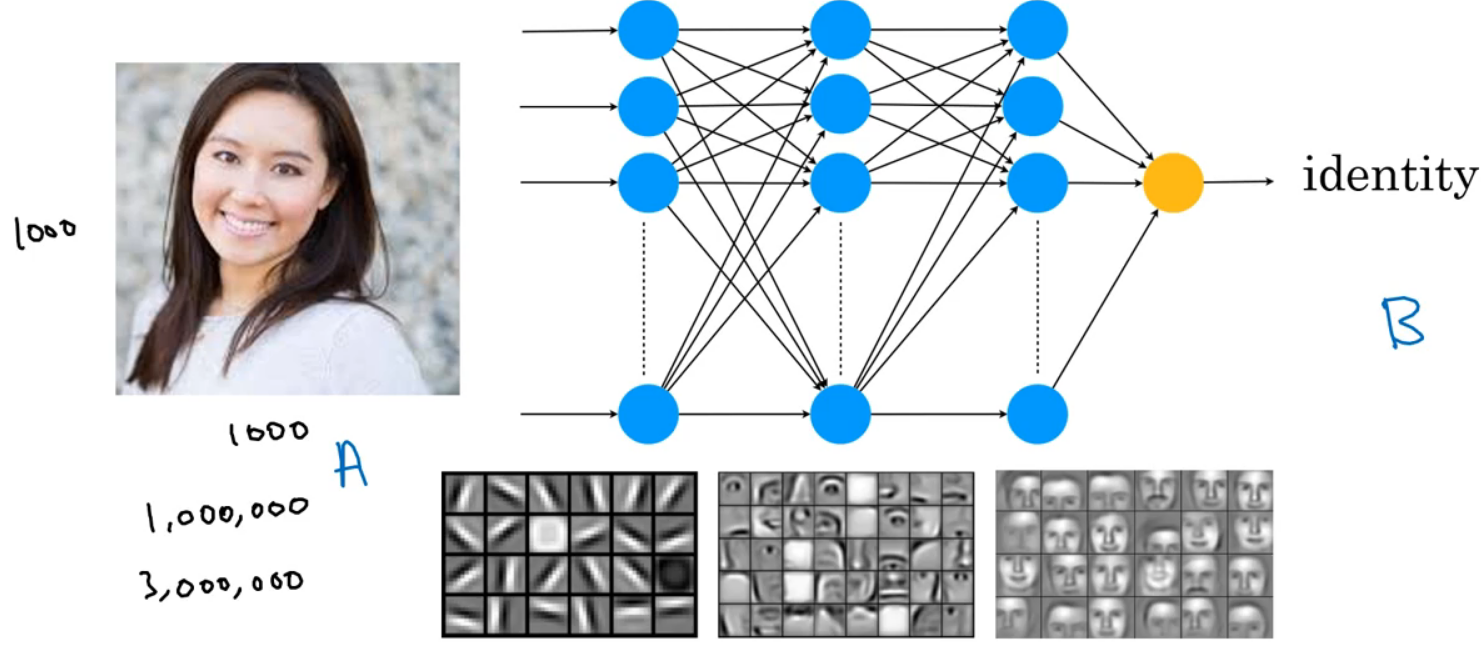
\includegraphics[scale=.225]{face-recognition-intro-3}
\end{frame}




\section{Survey of major AI application areas}
\begin{frame}{Computer Vision (1/3)}
	\begin{itemize}
		\item Image classification/Object recognition 
		\begin{center}
			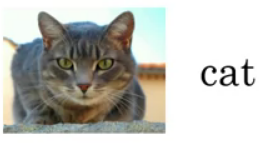
\includegraphics[scale=.4]{image-classification}	
		\end{center}
		\begin{itemize}
			\item Face recognition
			\begin{center}
				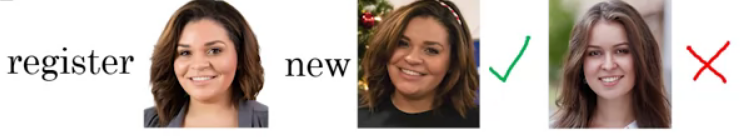
\includegraphics[scale=.35]{face-recognition}
			\end{center}
		\end{itemize}
	\end{itemize}
\end{frame}

\begin{frame}{Computer Vision (2/3)}
	\begin{itemize}
		\item Object detection
		\begin{center}
			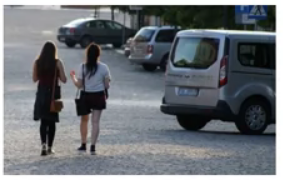
\includegraphics[scale=.4]{object-detection-1} \qquad 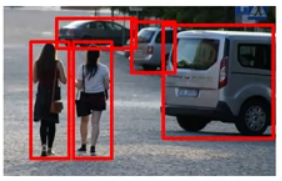
\includegraphics[scale=.4]{object-detection-2}
			\bigskip			
			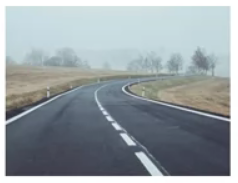
\includegraphics[scale=.4]{object-detection-3}	
		\end{center}
	\end{itemize}
\end{frame}

\begin{frame}{Computer Vision (3/3)}
	\begin{itemize}
		\item Image Segmentation
		\begin{center}
			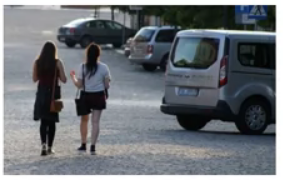
\includegraphics[scale=.4]{object-detection-1} \qquad 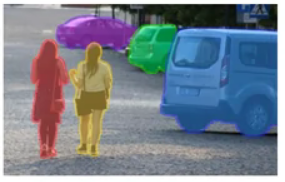
\includegraphics[scale=.4]{image-segmentation}	
		\end{center}
		\item Tracking
		\begin{center}
			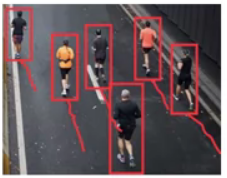
\includegraphics[scale=.4]{tracking}
		\end{center}
	\end{itemize}
\end{frame}

\begin{frame}{Natural Language Processing (1/7)}
	\begin{itemize}
		\item Text Classification
		
		\bigskip		
		
		\begin{tabular}{lcl}
			Email & $\longrightarrow$ & Spam/Non-Spam \\
			Product description & $\longrightarrow$ & Product category
		\end{tabular}
		\begin{itemize}
			\item Sentiment recognition
			
			\begin{tabular}{lcl}
				"The food was good"     & $\longrightarrow$ & 
\includegraphics[scale=.25]{four-stars}	\\
				"Service was horrible"  & $\longrightarrow$ & 
\includegraphics[scale=.25]{one-star}                      
			\end{tabular}
		\end{itemize}		

		\bigskip		
		
		\item Information retrieval 
			\begin{itemize}
				\item E.g., web search
			\end{itemize}
	\end{itemize}
\end{frame}


\begin{frame}{Natural Language Processing (2/7)}
	\begin{itemize}
		\item Name entity recognition 
		\begin{center}
			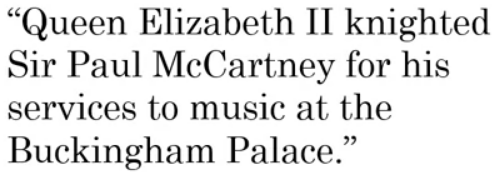
\includegraphics[scale=.25]{ner} \qquad 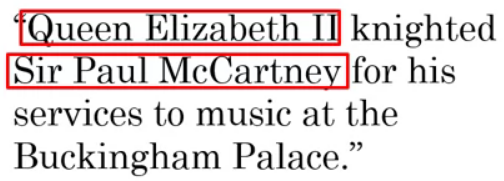
\includegraphics[scale=.25]{ner-2} \qquad 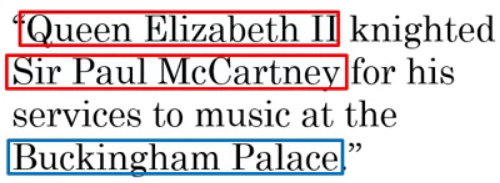
\includegraphics[scale=.25]{ner-3}
		\end{center}
		\item Machine translation \\
		"AI adalah listrik baru" $\Longrightarrow$ "AI is new electricity"
	\end{itemize}
\end{frame}

\begin{frame}{Natural Language Processing (3/7)}
	\begin{itemize}
		\item Others: parsing, part-of-speech tagging
		\begin{center}
			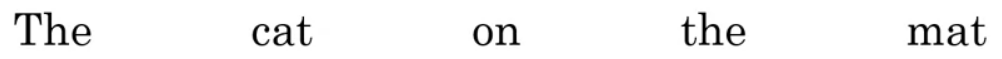
\includegraphics[scale=.25]{parsing-1} 	
		\end{center}
	\end{itemize}
\end{frame}

\begin{frame}{Natural Language Processing (4/7)}
	\begin{itemize}
		\item Others: parsing, part-of-speech tagging
		\begin{center}
			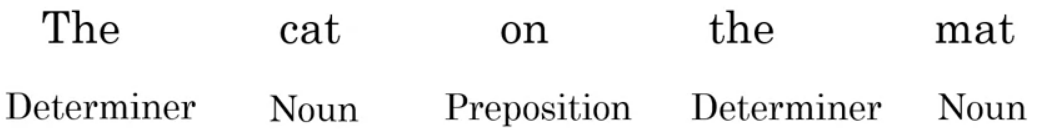
\includegraphics[scale=.25]{parsing-2} 	
		\end{center}
	\end{itemize}
\end{frame}

\begin{frame}{Natural Language Processing (5/7)}
	\begin{itemize}
		\item Others: parsing, part-of-speech tagging
		\begin{center}
			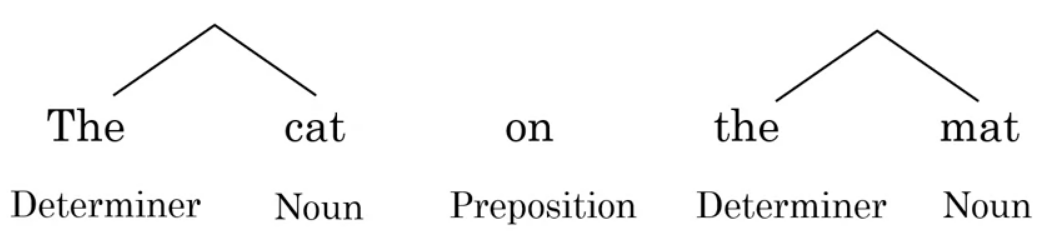
\includegraphics[scale=.25]{parsing-3} 	
		\end{center}
	\end{itemize}
\end{frame}

\begin{frame}{Natural Language Processing (6/7)}
	\begin{itemize}
		\item Others: parsing, part-of-speech tagging
		\begin{center}
			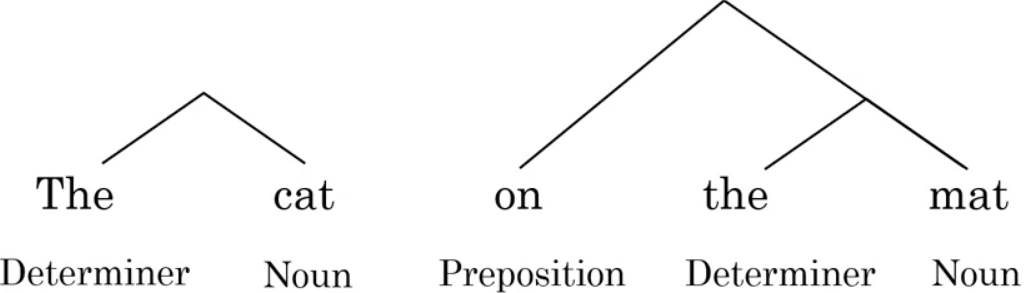
\includegraphics[scale=.25]{parsing-4} 	
		\end{center}
	\end{itemize}
\end{frame}

\begin{frame}{Natural Language Processing (7/7)}
	\begin{itemize}
		\item Others: parsing, part-of-speech tagging
		\begin{center}
			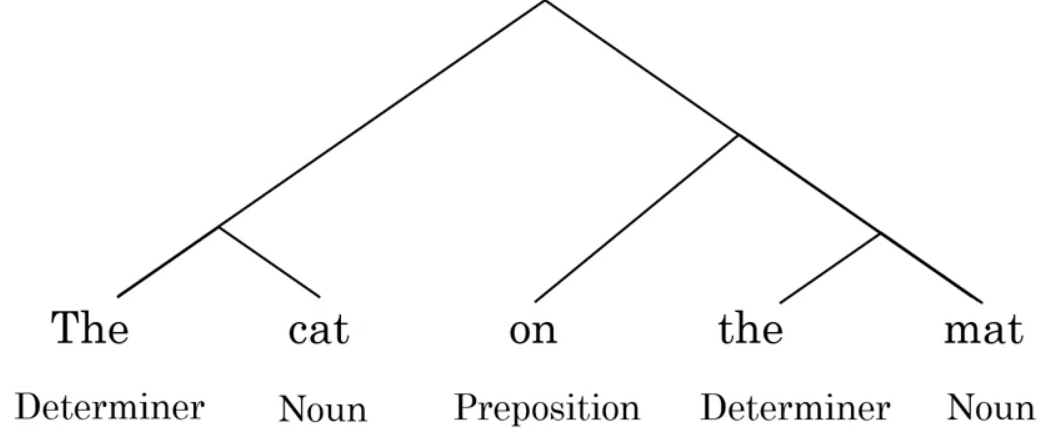
\includegraphics[scale=.25]{parsing-5} 	
		\end{center}
	\end{itemize}
\end{frame}

\begin{frame}{Speech (1/2)}
	\begin{center}
		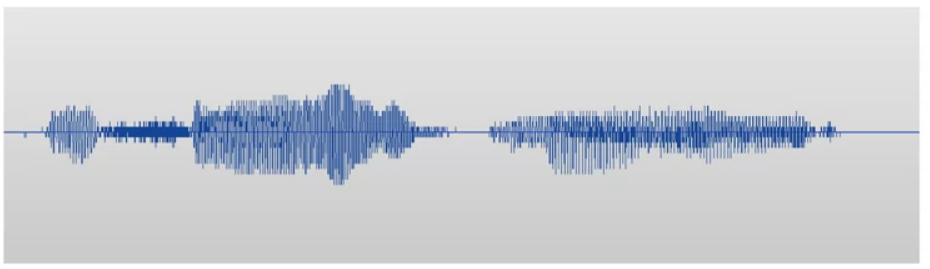
\includegraphics[scale=.25]{speech-1}
	\end{center}
	\begin{itemize}
		\item Speech recognition (speech-to-text) \\
		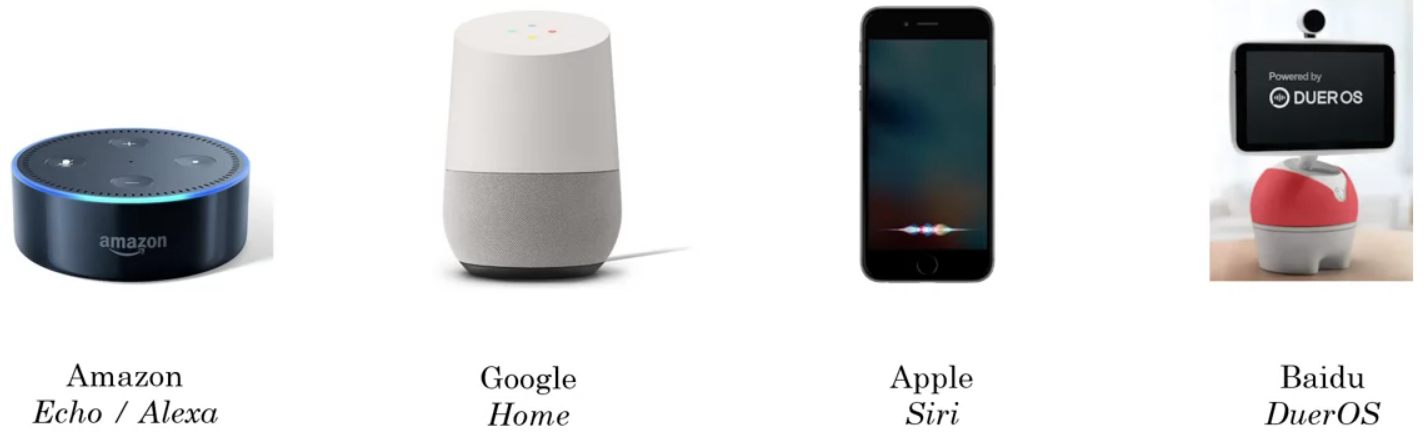
\includegraphics[scale=.2]{smart-speakers}
		\item Trigger word/wakeword detection \\
		Audio $\longrightarrow$ "Hey device"? (0/1)
	\end{itemize}
\end{frame}

\begin{frame}{Speech (2/2)}
	\begin{itemize}
		\item Speaker ID

		\bigskip

		\item Speech synthesis (text-to-speech, TTS)
		\begin{center}
			\texttt{The quick brown fox jumps over the lazy dog.}	
		\end{center}						
	\end{itemize}
\end{frame}

\begin{frame}{Robotics}
	\begin{itemize}
		\item Perception: figuring out what's in the world around you. \\
		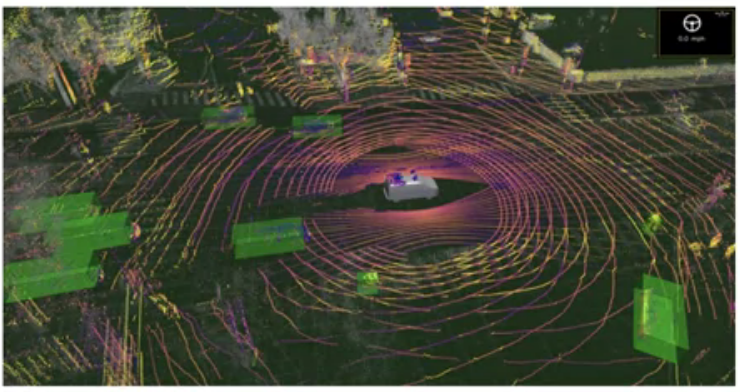
\includegraphics[scale=.2]{perception} \; 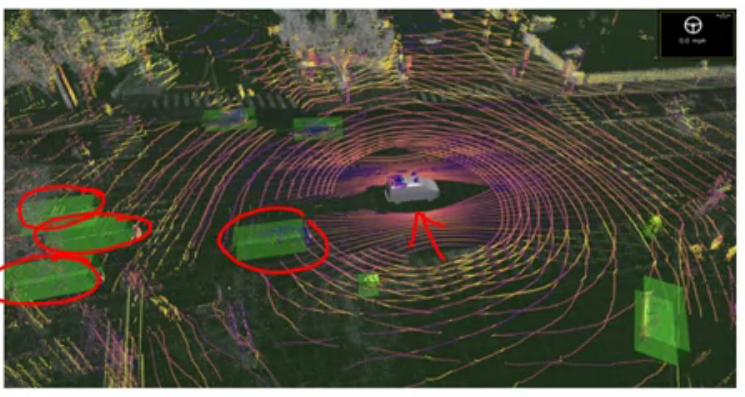
\includegraphics[scale=.2]{perception-2} \\
		\item Motion planning: finding a path for the robot to follow.
		\begin{center}
			\includegraphics[scale=.25]{motion-planning}	
		\end{center}
		\item Control: sending commands to the motors to follow a path
		
	\end{itemize}
\end{frame}


\begin{frame}{General machine learning}
	\begin{itemize}
		\item Unstructured data (images, audio, text)
		\includegraphics[scale=.225]{unstructed-data}
		\item Structured data
		\includegraphics[scale=.22]{structured-data}
	\end{itemize}	
\end{frame}

\begin{frame}{Unsupervised learning (1/2)}
	Clustering potato chip sales
	\begin{center}
		\includegraphics[scale=.25]{potato-chip-sales} \qquad \includegraphics[scale=.25]{potato-chip-sales-2}
	\end{center}
	
\end{frame}

\begin{frame}{Unsupervised learning (2/2)}
	\textbf{Unsupervised learning}:
	\begin{center}
		\textit{Given data (without any specific desired output labels), find something interesting about the data.}
	\end{center}
	
	\textbf{Another example of unsupervised learning:}
	
	\bigskip	
	
	Finding cats from unlabeled YouTube videos
	\begin{center}
		\includegraphics[scale=.25]{google-cats}
	\end{center}	
\end{frame}

\begin{frame}{Transfer learning}
	\begin{center}
		\includegraphics[scale=.225]{transfer-learning}
	\end{center}
	\begin{center}
	Learn from task A, and use knowledge to help on task B	
	\end{center}	
\end{frame}

\begin{frame}{Reinforcement learning (1/2)}
	\begin{center}
		\includegraphics[scale=.325]{reinforcement-learning}
	\end{center}
	Use a "reward" signal to tell the AI when it is doing well or poorly. It automatically learns to maximize its rewards.
\end{frame}

\begin{frame}{Reinforcement learning (2/2)}
	\begin{center}
		\includegraphics[scale=.325]{reinforcement-learning-2}
	\end{center}
	Use a "reward" signal to tell the AI when it is doing well or poorly. It automatically learns to maximize its rewards.
\end{frame}

\begin{frame}{GANs (Generative Adversarial Network)}
	\begin{center}
		Synthesize new images from scratch~\citep{karras2017progressive}
	\end{center}
	\begin{center}
		\includegraphics[scale=.25]{GANs}
	\end{center}		
\end{frame}

\begin{frame}{Knowledge Graph (1/4)}
	\begin{center}
		\includegraphics[scale=.35]{leonardo-da-vinci}
	\end{center}
	
\end{frame}

\begin{frame}{Knowledge Graph (2/4)}
	\begin{center}
		\includegraphics[scale=.35]{ada-lovelace}
	\end{center}
	
\end{frame}

\begin{frame}{Knowledge Graph (3/4)}
	\begin{center}
		\includegraphics[scale=.35]{knowledge-graph-1}
	\end{center}
\end{frame}

\begin{frame}{Knowledge Graph (4/4)}
	\begin{center}
		\includegraphics[scale=.35]{knowledge-graph-2}
	\end{center}
\end{frame}

\section{MK Pilihan Jalur Komputasi Cerdas}
\begin{frame}{Mata Kuliah Pilihan}
	\begin{table}[!ht]
		\centering
		\begin{tabular}{|l|l|l|l|}
			\hline
			\multicolumn{1}{|c|}{Kode} & \multicolumn{1}{c|}{Nama MK} & \multicolumn{1}{c|}{SKS} & \multicolumn{1}{c|}{Prasyarat} \\
			\hline
			IN056 & Teknik Kompilasi        & 3+1 & IN035 MatDis \\
			\hline
			IN068 & Competitive Programming & 3+1 & - \\
			\hline
			IN075 & Sistem Pakar            & 3   & - \\
			\hline
			IN086 & Temu Pengetahuan        & 3+1 & - \\
			\hline
			IN074 & Pembelajaran Mesin      & 3+1 & IN060 PKB \\
			\hline
			IN084 & Pengantar Temu Balik Informasi & 3+1 & - \\
			\hline
			IN085 & Pemrosesan Bahasa Alami        & 3   & - \\
			\hline
			IN039 & Topik Lanjut Komputasi Cerdas  & 3+1 & - \\
			\hline 
		\end{tabular}
	\end{table}
\end{frame}



%\noindent\fbox{%
%    \parbox{\textwidth}{%
%        The quick brown fox jumps right over the lazy dog. 
%    }%
%}











%\begin{frame}{Blocks}
%\begin{block}{Block Title}
%You can also highlight sections of your presentation in a block, with it's own title
%\end{block}
%\begin{theorem}
%There are separate environments for theorems, examples, definitions and proofs.
%\end{theorem}
%\begin{example}
%Here is an example of an example block.
%\end{example}
%\end{frame}


% All of the following is optional and typically not needed. 
\appendix
\section<presentation>*{\appendixname}
\subsection<presentation>*{For Further Reading}

\begin{frame}[allowframebreaks]
  \frametitle<presentation>{Daftar Pustaka}
    {\footnotesize
    \bibliographystyle{apalike}
    \bibliography{references}
    }    
\end{frame}




%\makeatletter % to change template
%    \setbeamertemplate{headline}[default] % not mandatory, but I though it was better to set it blank
%    \def\beamer@entrycode{\vspace*{-\headheight}} % here is the part we are interested in :)
%\makeatother

\begin{frame}[plain]
		\centering\includegraphics[scale=0.5]{Logo-Maranatha-Untuk-Belakang-02}	
\end{frame}

\end{document}


